\subsubsubsubsection{Direction}
\begin{figure}[h]
\centering
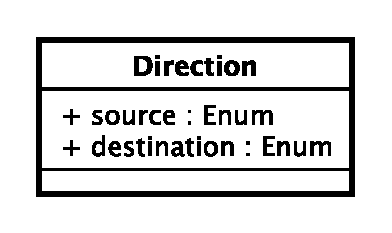
\includegraphics[scale=0.6,keepaspectratio]{images/solution/direction.eps}
\caption{App::Reactive::Direction}
\label{fig:sd-app-direction}
\end{figure}
\FloatBarrier
\begin{itemize}
  \item \textbf{Description} \\
    It represents the direction. 
  \item \textbf{Attribute}
  \begin{itemize}
    \item \texttt{- source: Enum} \\
The source from which an entity arrives. It has four possible
values \{ north, south, east, west \}
    \item \texttt{- destination: Enum} \\
The destination where the entity is directed. It has the same possible
values of source.
  \end{itemize}
\end{itemize}
